% !TeX spellcheck = en_US
\section*{Test run of detrnn.py}

Test report

by E. Marquer, 2018/04/30, Synalp and Université de Lorraine

\subsection{Abstract}

Test to do a complete run on 50 epoch, with GPU, of the basic model of
DetRNN.

\subsection{Paradigm}

This test run of \emph{detrnn.py}, with INFO level log output, loss by
percentile and vbpc by epoch, will be executed with \emph{cuda}, for 50
epochs.

The test is done with branch
\href{https://gitlab.inria.fr/emarquer/awd-lstm-lm/tree/reimplement}{reimplement},
an allocated time of 76h, not interactive

Run time was estimated for 50 epochs according to the results for 4
epochs (see
\href{https://gitlab.inria.fr/emarquer/awd-lstm-lm/blob/master/docsEsteban/testReports/2018-04-27_test_run_detrnn.md}{2018-04-27\_test\_run\_detrnn.md}):

\begin{quote}
(5h 33min / 4 epoch) * 50 epoch = 4162.5min = 69h 22min 30s
\end{quote}

With a security margin of 10h, partially due to reduced batchsize, run
time is 80h.

\emph{/!\textbackslash{} Had to reduce batchsize down to 40 because of
memory errors /!\textbackslash{}}

\subsubsection{Node}

OAR\_JOB\_ID=155659 with GPU

Job start time: 2018-04-30 12:02:08

Estimated job stop time: 2018-05-03 16:02:08

Command used:
\lstinline!bash oarsub -q production -p "GPU <> 'NO'" -l "nodes=1,walltime=80:00:00" ~/awd-lstm-lm/rundet.sh!

\newpage
\subsection{Results}

Total run time for 50 epochs: with real stop time of 2018-05-02
17:16:56, the total run time of the training is aproximately 53h (2days
5h), corresponding to a little more than an hour per epoch.

BPC-wise, the DetRNN hardly goes under 2.7 even after 50 epoch, with a
change of 0.5 BPC in the last 30 epochs.

We can postulate that enven after 200 epoch, the DetRNN will not have a
BPC under 2.

\subsubsection{Plot}

\paragraph{BPC/fraction of corpus}

BPS per fraction of the corpus (an interval of 1 correspond a complete
corpus, or an epoch).

\begin{figure}[ht]
\centering
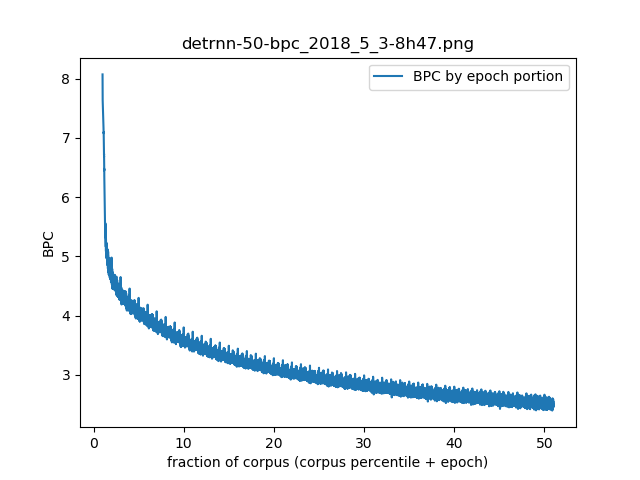
\includegraphics{parts/appendix/reports-gmsnn/docs_esteban-latex/test_reports/detrnn-50/detrnn-50-bpc_2018_5_3-8h47.png}
\caption{BPC}
\end{figure}

\newpage
\paragraph{ValBPC/epoch}

Mean BPC over the epoch, at the end of each epoch.

\begin{figure}[ht]
\centering
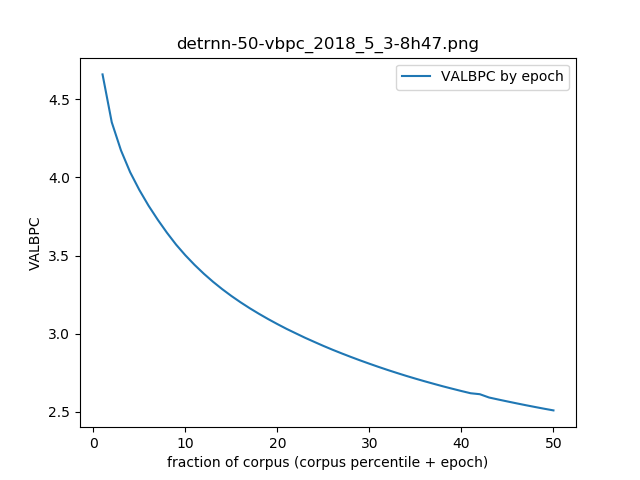
\includegraphics{parts/appendix/reports-gmsnn/docs_esteban-latex/test_reports/detrnn-50/detrnn-50-vbpc_2018_5_3-8h47.png}
\caption{ValBPC}
\end{figure}

\newpage
\paragraph{Loss}

Loss per fraction of the corpus (an interval of 1 correspond a complete
corpus, or an epoch).

\begin{figure}[ht]
\centering
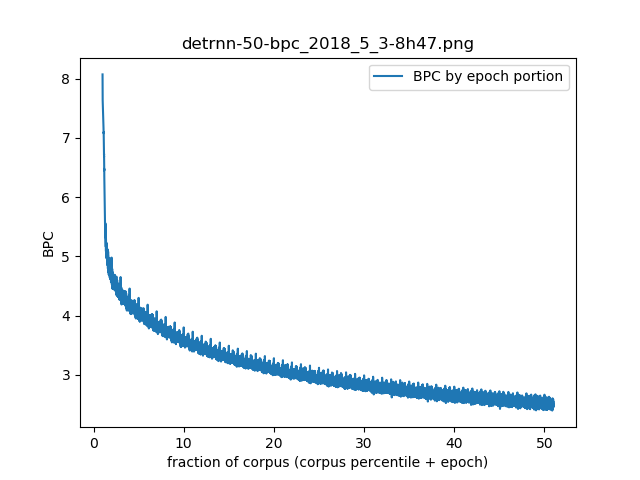
\includegraphics{parts/appendix/reports-gmsnn/docs_esteban-latex/test_reports/detrnn-50/detrnn-50-bpc_2018_5_3-8h47.png}
\caption{Loss}
\end{figure}

\subsubsection{Logs}

The log is available at 
\href{https://gitlab.inria.fr/emarquer/awd-lstm-lm/blob/reimplement/logs/detrnn-50_2018_4_30-12h2.log}{https://gitlab.inria.fr/emarquer/awd-lstm-lm/blob/reimplement/logs/detrnn-50\_2018\_4\_30-12h2.log}.

\subsection{Potential ameliorations \& next steps}

Next step is to test the growing model.
